\section{Sistemas de gestión curricular}
Un CMS \footnote{de sus siglas en inglés, Curriculum Management System, que significa sistema de gestión curricular} es un aplicación automatizada que apoya todo el proceso curricular, desde la planificación hasta la implementación y evaluación. Posee una interfaz única y cohesiva en línea que permite proponer, crear, evaluar, revisar, aprobar y aplicar cursos, programas y competencias.

Curriculum es una mezcla sofisticada de estrategias educativas, contenido del curso, resultados de aprendizaje, experiencias educativas y evaluación\citep{harden2001amee}. Esta visión amplia de un CMS se deriva del ambiente actual de educación elemental y secundaria que es impulsado por los estándares de contenido de cursos obligatorios federales y estatales, y la necesidad de auditorías continuas de currículo\citep{west2000technology}.

En los enfoques actuales del desarrollo de Curriculum por lo general gira en torno a los comités curriculares. Un comité curricular departamental comienza el proceso de desarrollo curricular considerando como entrada cualquiera de los aspectos mostrados en la figura \ref{diseno_curricular}.

\begin{figure}[H]
\centering
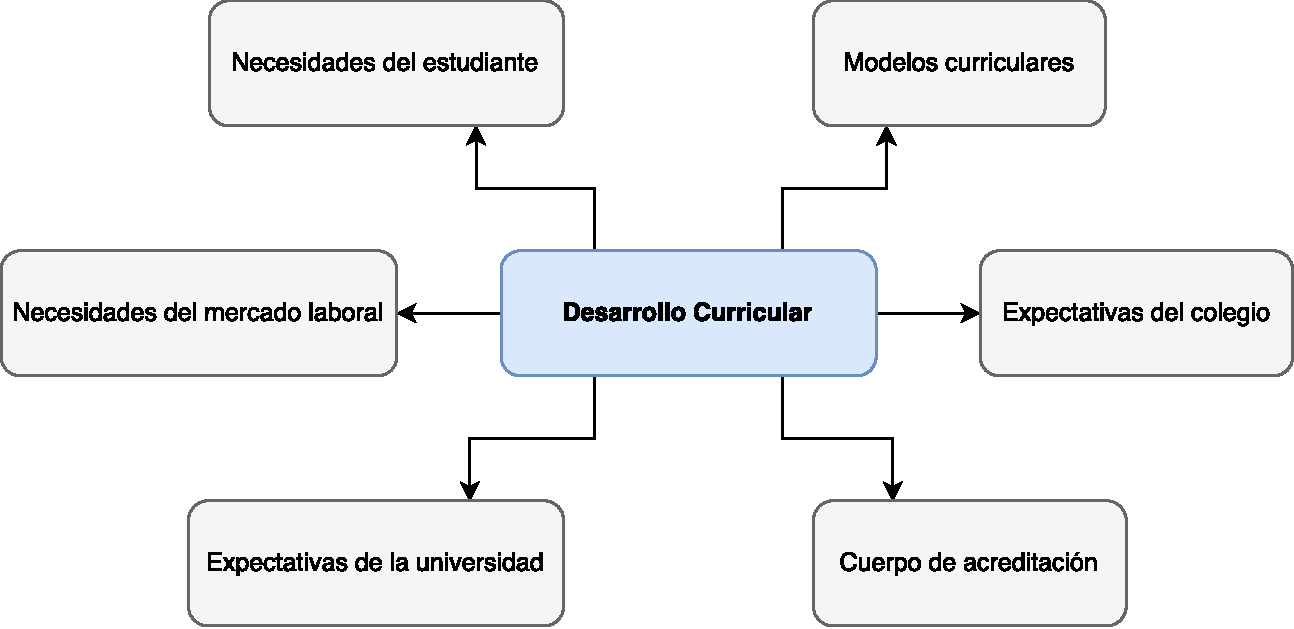
\includegraphics[width=125mm,scale=1]{Figuras/diseno_curricular}
\caption{Esquema de diseño curricular y sus variables determinantes.}
  \label{diseno_curricular}
\end{figure}


Dichos aspectos, sin embargo, sólo se consideran en un alto nivel de abstracción basado en la comprensión tácita de los miembros del comité sobre la disciplina.